%!TEX root = main.tex
\Lesson{Символы}\label{Less:symbols}

\section{Символы и~их значения}%
До сих пор мы имели дело с~константами и~символами-идентификаторами, игравшими роль переменных или имён функций. При~этом символ должен был быть связан с~каким-либо значением~--- константой или функцией, в~противном случае возникала ошибка.

Если мы собираемся производить символьные преобразования, то нам вовсе не~обязательно требовать чтобы символы имели какие-то конкретные значения. Например, если мы рассматриваем преобразование $(a + b)^2 = a^2 + 2ab + b^2$, нам не~важно, чему равны $a$ и~$b$~--- мы работаем с~формальными символами.

Язык \Scheme позволяет работать с~выражениями, не~вычисляя их. Для этого служит форма \s{quote}\index{Racket!базовые формы!quote@\s{'} (\s{quote})}:

\begin{example}{Попробуем ввести выражение с~неопределёнными символами и~получим сообщение об~ошибке.

Использование формы \s{quote} оставляет выражение невычисленным.}
\REPLin
  {(+ a b)}

\REPLerror{reference to an identifier before its definition: a}

\REPL
  {(quote (+ a b))}
  {(+ a b)}
\end{example}

Знак кавычки \s{'} является кратким обозначением формы \s{quote}:

\begin{example}{В то время, как первый элемент списка \s{(list a 'a)} вычисляется, второй остаётся в~виде символа.}
\REPLin
  {(define a 8)}

\REPL
  {(list a 'a)}
  {(8 a)}
\end{example}

Выражение, взятое в~кавычки, можно вычислить с~помощью функции \sbi{eval}:

\begin{example}{Выражение \s{x} содержит в~себе невычисленную сумму. Применение функции \s{eval} снимает кавычки и~вычисляет его, применяя все известные интерпретатору определения.}
\REPLin
  {(define x '(+ a 5))}

\REPL
  {x}
  {(+ a 5)}

\REPL
  {(eval x)}
  {13}
\end{example}

По существу, функция \s{eval} является вызовом интерпретатора \Scheme для введённого выражения:

\begin{example}{Выражение \s{proc} содержит в~себе определение функции.

Это определение не~выполняется,  и~символ \s{1+} является неопределённым.

Функция \s{eval} интерпретирует  выражение \s{proc}, как программу \Scheme.}
\begin{ExampleCode}
(define proc
  '(define (1+ x)
       (+ 1 x)))
\end{ExampleCode}

\REPL
  {proc}
  {'(define (1+ x) (+ 1 x))}

\REPLin
  {(1+ 2)}

\REPLerror{1+: undefined;\newline cannot reference an identifier before its definition}

\REPLin
  {(eval proc)}

\REPL
  {(1+ 2)}
  {3}
\end{example}

Часто бывает нужно оставив выражение невычисленным, вычислить некоторые его части. Для этого служит форма \s{quasiquote} или символ \s{`} (обратная кавычка).\index{Racket!базовые формы!quasiquote@\s{`} (\s{quasiquote})} Эта форма работает так же, как и~\s{quote}, но часть выражения можно заменить его значением, если поместить его в~форму \s{unquote} или поставить перед ним символ \s{,} (запятая).\index{Racket!базовые формы!unquote@\s{,} (\s{unquote})}

\begin{example}{Обратная кавычка позволяет вычислять только ту часть выражения, которая следует за~знаком запятой. Всё остальное остаётся невычисленным.}
\REPL
  {`(a ,(+ 2 3) (+ 1 2))}
  {'(a 5 (+ 1 2))}
\end{example}

\begin{example}{Комбинация символов \s{,@} не~просто вычисляет подвыражение, но и~убирает лишние скобки.}
\REPLin
  {(define x '(a b c))}

\REPL
  {`(+ ,x)}
  {'(+ (a b c))}

\REPL
  {`(+ ,@x)}
  {'(+ a b c)}
\end{example}

Кавычки \s{quote}, \s{quasiquote} и~функция \s{eval} являются мощным инструментом~--- они дают нам способ строить выражения, которые работают с~другими выражениями. Таким образом, в~функциональных языках стирается принципиальное различие между программой и~данными, поскольку данные сами могут играть роль программы.


%=============================================================
% Формальные функции
%=============================================================

\section[4]{Абстрактные типы данных и формальные~функции}%
\index{тип!абстрактный}%
На предыдущем занятии мы встретились с понятием абстрактного типа данных. Экземпляры таких типов образуются с помощью функций-конструкторов, часто не производящих никаких вычислений, и возвращающих данные <<упакованными>> в определённую структуру. Для того чтобы отличать величины принадлежащие разным абстрактным типам, необходим идентификатор типа, например, предикат, отличающий величины определённого типа от прочих. Доступ к элементам такой структуры осуществляется функциями-селекторами. Кроме использования функций-селекторов, получить доступ к элементам величины абстрактного типа позволяет техника сопоставления с образцом. Примером абстрактного типа является точечная пара с конструктором \s{cons}, селекторами \s{car} и \s{cdr} и идентифицирующим предикатом \s{pair?}.


В языке \Scheme для создания новых абстрактных типов служат \index{функция!формальная}\emph{формальные функции}, которые, не~производя никаких вычислений, возвращают в~качестве результата заквотированное выражение, обозначающее их аппликацию.

Объявляются формальные функции формой \sfi{define-formal}.

\begin{example}{%
Декларируем функции \s{f} и \s{g}, как формальные. Причём \s{f} может принимать произвольное количество аргументов, а \s{g} является бинарной. Результатом аппликации формальной функции является список.}
\REPLin
  {(define-formal f (g 2)}
\REPL
  {(f 1)}
  {(f 1)}
\REPL
  {(f (g 'x 'y) 'z)}
  {(f (g x y) z)}
\REPL
  {(is (f 'x) list?)}{#t}
\end{example}

\begin{example}{%
При объявлении формальной функции с сименем \s{id} создаются
\begin{itemize}
\item идентифицирующий предикат \s{id?}, отличающий аппликацию этой функции от других списков, 
\item шаблон для этой функции \s{(id ...)} 
\item и комбинатор для абстрактного типа \s{id:}.
\end{itemize}}
\REPL{(is (f 1) f?)}{#t}
\REPL{(is (f 1) g?)}{#f}
\smallskip
\begin{ExampleCode}
> ((/. (f a b) --> a) 
   (f 1 2))
\end{ExampleCode}
\REPLout{1}
\smallskip
\begin{ExampleCode}
> ((/. (f (g a b) c) --> b) 
   (f (g 1 2) 3))
\end{ExampleCode}
\REPLout{3}
\begin{ExampleCode}
> (is (f (g 1 2) 3)
      (f: (g: Int Int) Int))
\end{ExampleCode}
\REPLout{#t}
\end{example}

\begin{Assignment}
а) Напишите простейшее определение формальной функции \s{f}, удовлетворяющей спецификации:
\begin{Specification}
(test 
  (f 'x)                ==> '(f x)
  (f 1 2 3)             ==> '(f 1 2 3)
  (map f '(1 2 3))      ==> '((f 1) (f 2) (f 3))
  (foldr f 'x '(a b c)) ==> '(f a (f b (f c x))) )
\end{Specification}

б) Напишите функцию \fun{hold}{s}, которая бы делала формальной функцией любой указанный символ. 
\begin{Specification}
(test 
 ((hold 'g) 1 2 3)             ==> '(g 1 2 3)
 (map (hold '+) '(1 2) '(3 4)) ==> '((+ 1 3) (+ 2 4)))
\end{Specification}

Сможете ли вы обойтись без~использования форм \s{quote} и~\s{quasiquote} при~решении этой задачи?
\end{Assignment}


\section{Программы и~данные}%
В качестве развёрнутого практического примера, использования заквотированных выражений и абстрактных данных, рассмотрим задачу расчёта импеданса электрических цепей переменного тока. Мы будем рассматривать цепи, содержащие только сопротивления, индуктивности и~ёмкости.

Как известно, в~случае переменного тока, каждый из~рассмотренного нами типов элементов имеет полное сопротивление~--- \emph{импеданс} $Z$, выражаемый комплексным числом. Действительная часть этого числа отражает активное сопротивление элемента, а мнимая --- реактивное. Для заданной частоты переменного тока в~цепи $\omega$ импедансы сопротивления $R$, индуктивности $L$, и ёмкости $C$ вычисляются следующим образом:
$$Z_R = R,\qquad Z_C = \frac{1}{i \omega C},\qquad Z_L = i\omega L.$$
Кроме этого, можно вычислить импедансы для последовательного и~параллельного соединения элементов цепи:
$$Z_\text{посл} = Z_1 + Z_2 +...,\qquad  Z_\text{парал}= \left(\frac1{Z_1} + \frac1Z_2 +...\right)^{-1}.$$

Для представления электрических схем нужна форма записи, как для элементов, так и~для возможных типов их соединения. Мы будем использовать следующие обозначения:

\begin{itemize}
 \item[] \s{(R $x$)} для сопротивления в~$x$ ом;

 \item[] \s{(L $x$)} для катушки индуктивностью $x$ генри;

 \item[] \s{(C $x$)} для конденсатора ёмкостью $x$ фарад;

 \item[] \s{(-- $el_1$ $el_2$ ...)} для последовательного соединения элементов;

 \item[] \s{(|| $el_1$ $el_2$ ...)} для параллельного соединения.
\end{itemize}

Определим для элементов цепи соответствующие формальные функции:
\begin{Definition}
(define-formal 
  (R 1) (C 1) (L 1) -- ||)
\end{Definition}
Так, например, можно представить в~виде символьного выражения цепь, изображённую на~рисунке:

\medskip
\begin{tabular}{ll}%
\label{circuit}
\begin{SchemeCode}
(define circuit
  (-- (R 10)
      (|| (L 0.5)
          (-- (R 3)
              (C 1e-5)))))
\end{SchemeCode}
&
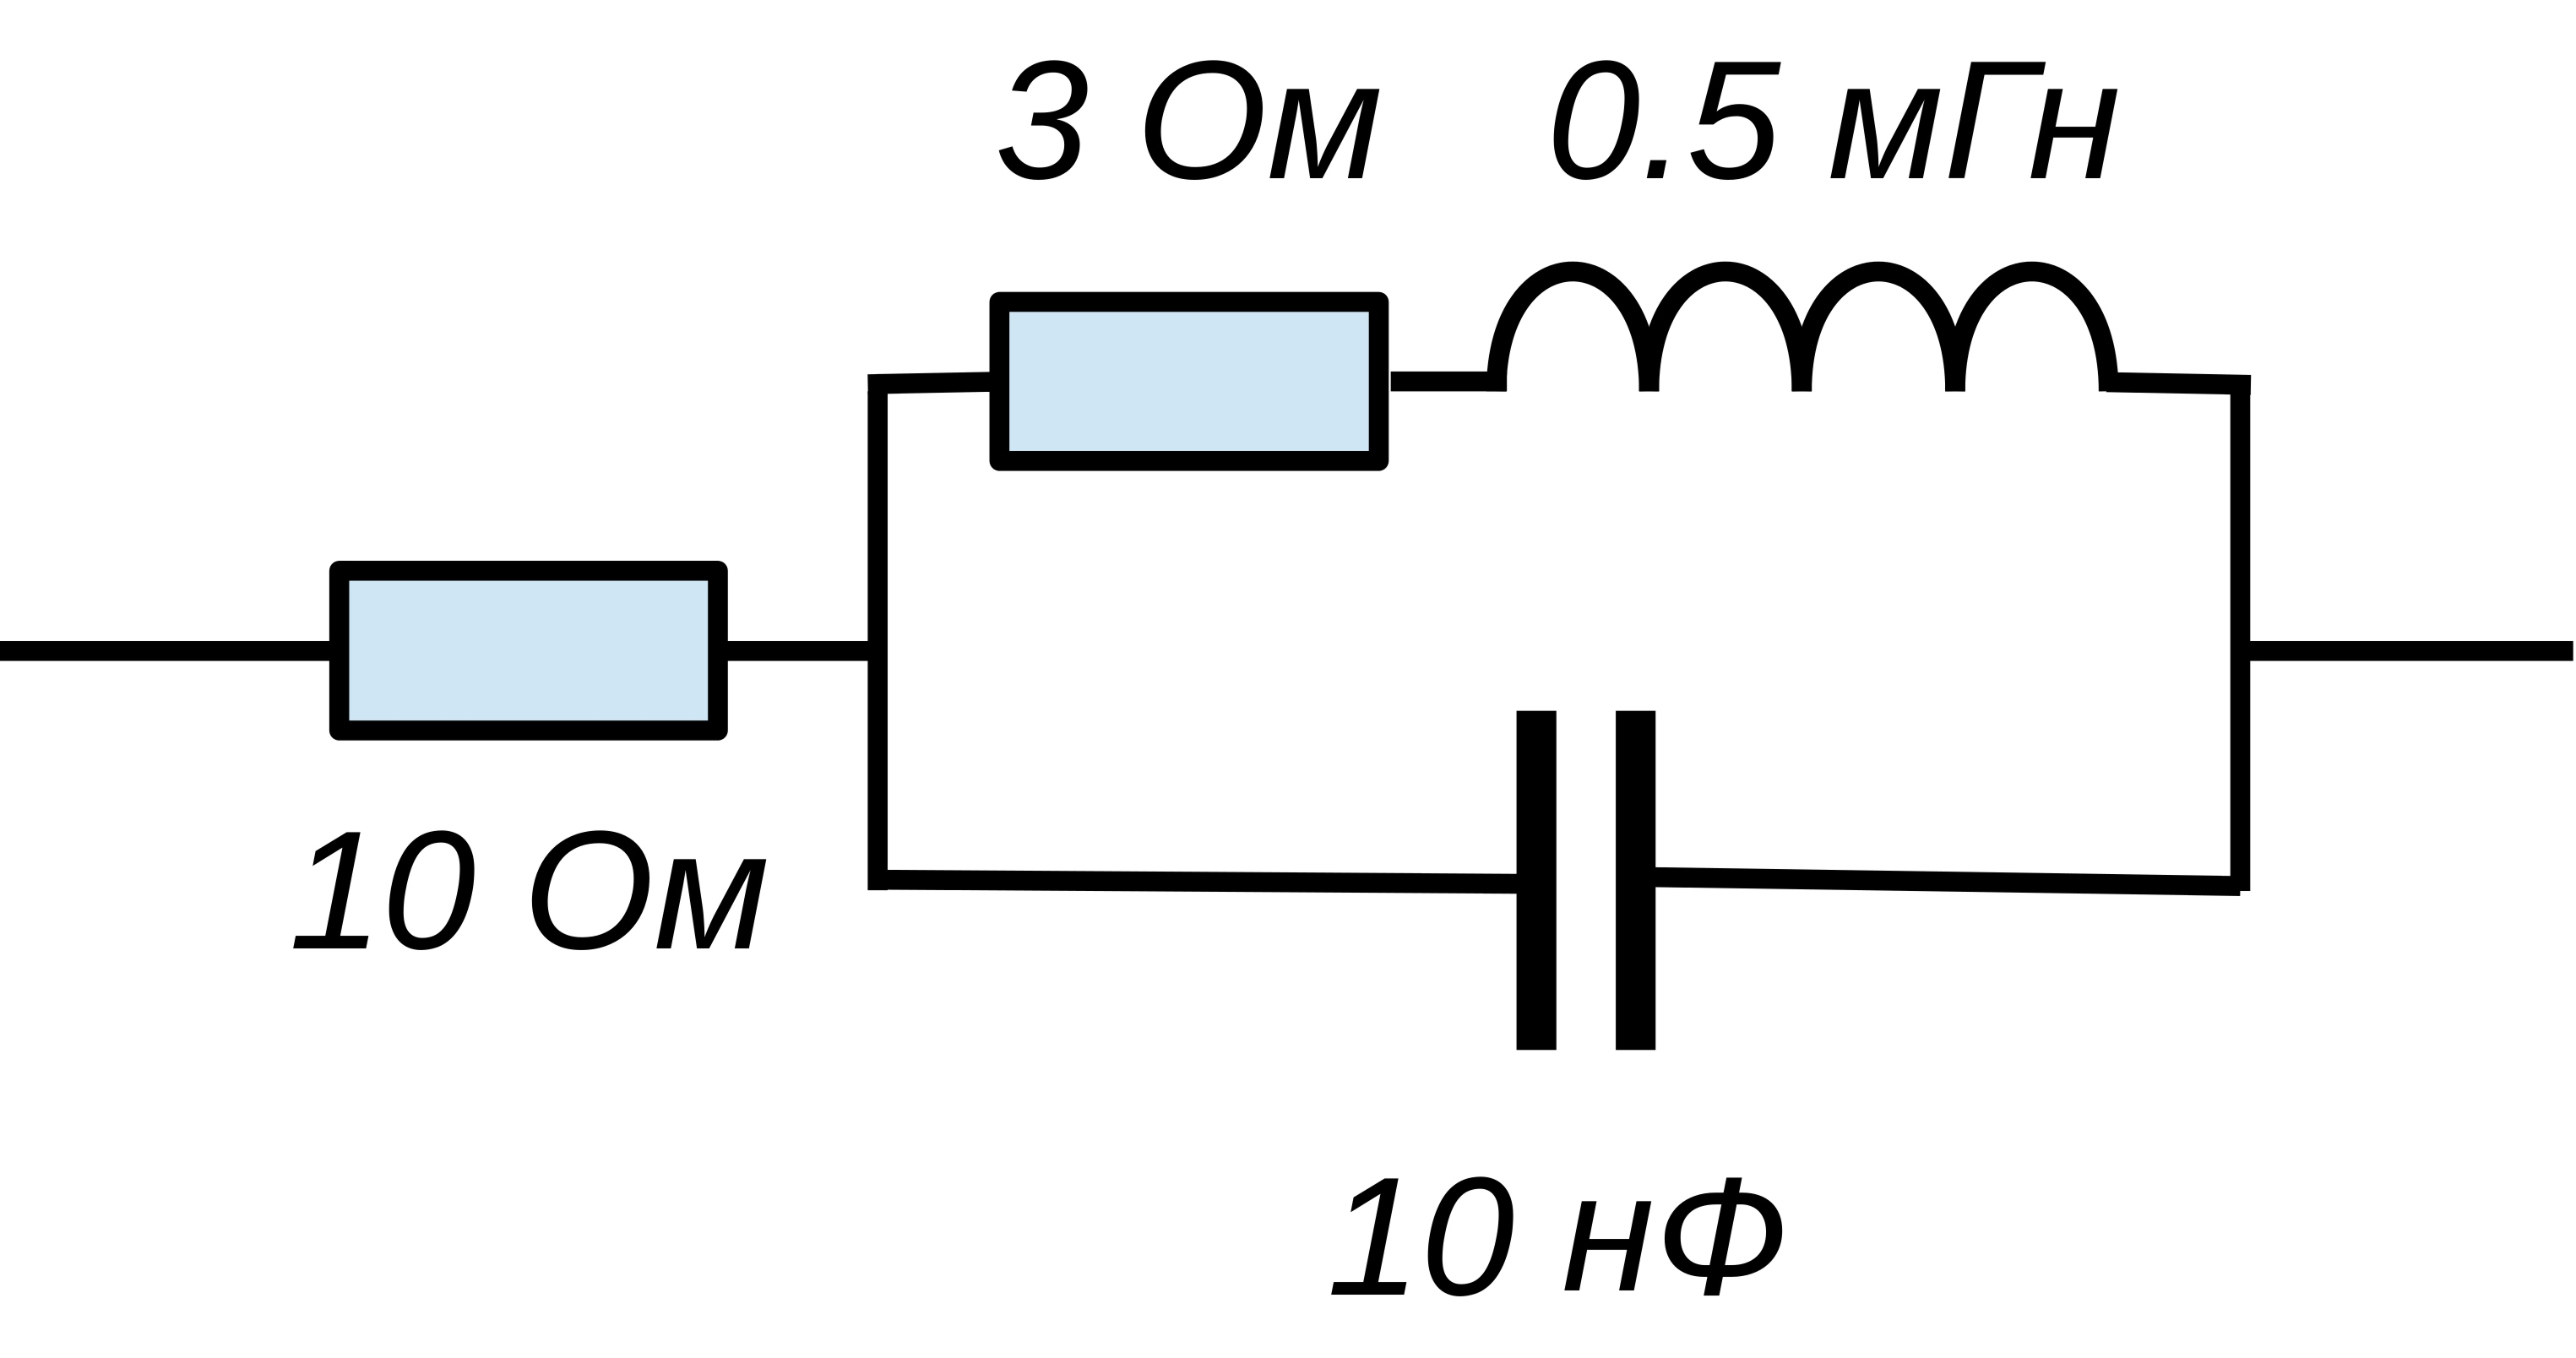
\includegraphics[width=0.4\textwidth,viewport=0 40 139 71]{../figures/circuit.pdf}
\end{tabular}
\newpage

\noindent Сразу же опишем и тип для корректной электрической цепи:
\begin{Definition}
(define-type Circuit
  (R: positive?)
  (C: positive?)
  (L: positive?)
  (--: Circuit ..)
  (||: Circuit ..))
\end{Definition}

Таким образом, мы определили язык, пригодный для описания простых электрических цепей. Теперь нужно научиться его интерпретировать и производить расчёты. Интерпретатор, который мы хотим создать, должен по заданной цепи строить функцию, вычисляющую импеданс цепи $Z$ для заданной частоты $\omega$. Так как частота должна быть положительным действительным числом, а импеданс выражается комплексным, то мы можем записать сигнатуру и <<скелет>> функции-интерпретатора \s{impedance} следующим образом:

\begin{SchemeCode}[emph={cir,w}]
(:: impedance (Circuit -> (positive? -> complex?))
 (define (impedance cir)
   (lambda (w) ...)))
\end{SchemeCode}

В теле \lmфункции нужно определить, как вычисляются импеданс элементов и соединений. Это нетрудно сделать с помощью сопоставления с образцом. Определим вспомогательную функцию \s{Z}, которая и будет производить это сопоставление:
\begin{SchemeCode}[emph={cir,w,r,c,l}]
(define Z 
  (/. (R r) --> r
      (C c) --> (/ -i c w)
      (L l) --> (* +i l w)
      (-- x ...) --> (sum Z x)
      (|| x ...) --> (/ (sum 1/Z x))))
\end{SchemeCode}
В свою очередь, функция \s{impedance} будет возвращать результат действия функции \s{Z} на цепь \lex{cir}.

Здесь мы постарались максимально чётко выразить способ вычисления через функцию \s[emph={f,lst}]{(sum f lst)}, вычисляющую сумму значений функции \lex{f} на элементах списка \lex{lst}.

Определим, для начала, как мы будем считать импедансы элементов:

\begin{Definition}[emph={x}]
; R :: Num \arrow Num
(define (R x) x)

; L :: Num \arrow Lit
(define (L x) `(* +i w ,%\lexical x%))

; C :: Num \arrow Lit
(define (C x) `(/ -i w ,%\lexical x%))
\end{Definition}

Обратите внимание на~то, что используя кавычки, мы можем ввести в~наши формулы неизвестную пока переменную \s{w}, обозначающую частоту переменного тока. При~этом, мы вычисляем переданные в~качестве аргументов номиналы \lex{x}. Посмотрим, как реагирует на~наши определения интерпретатор:
\REPL
  {(list (R 10) (L 0.5) (C 0.001))}
  {(10 (* 0+1i w 0.5) (/ 0-1i w 0.001))}
\noindent Как и~ожидалось, он возвращает символьные выражения для импедансов.

Опишем теперь, каким образом посчитать импедансы для различных соединений. Для последовательного соединения всё просто: мы превращаем его в~сумму.
\begin{Definition}[emph=z]
; -{-} :: Lit ... \arrow Lit
(define (-- . z) `(+ ,@%\lexical z%))
\end{Definition}
\noindent При~этом, мы используем символ \s{,@} затем, чтобы список аргументов не~был окружён лишними скобками:
\REPL
  {(-- 'a 'b 'c)}
  {(+ a b c)}

Формула для параллельного соединения несколько сложнее:
\begin{Definition}[emph={x,z}]
; || :: Lit ... \arrow Lit
(define (|| . z)
  `(/ 1 (+ ,@(map (lambda (x) `(/ 1 ,%\lexical x%)) z))))
\end{Definition}

Здесь мы сначала создаём список из~обратных импедансов, приписывая к~каждому из~них слева символы деления и~единицу. Посмотрим, что делает исполняемый участок кода:
\REPL
  {(map (lambda (x) `(/ 1 ,x)) '(a b c))}
  {((/ 1 a) (/ 1 b) (/ 1 c))}
\noindent Затем мы встраиваем этот список в~сумму и~делим на~неё единицу. Таким образом, мы получаем нужную нам формулу:
\REPL
  {(|| 'a 'b 'c)}
  {(/ 1 (+ (/ 1 a) (/ 1 b) (/ 1 c)))}

Теперь можно «вычислить» импеданс нашей сложной цепи:
\REPLin
  {(eval circuit)}
\begin{mREPLout}
   (+ 10 (/ 1 (+ (/ 1 (* 0+1i w 0.5))
         (/ 1 (+ 3 (/ 0-1i w 1e-5))))))
\end{mREPLout}
\noindent Как видите, мы получили в~качестве результата формулу, по~которой можно рассчитать импеданс сети для заданной частоты \s{w}. Создадим для этого расчёта функцию \s{impedance}:

\begin{Definition}[emph={w,circ}]
; impedance :: Lit \arrow Lit
(define (impedance circ)
  `(lambda (w) ,(eval circ)))
\end{Definition}

Здесь мы собираем нужную нам функцию, пока не~вычисляя её, для того, чтобы можно было посмотреть, что мы будем вычислять. Например, для нашей цепи мы получим функцию:
\REPLin
  {(impedance circuit)}
\begin{mREPLout}
  (lambda (w)
    (+ 10 (/ 1 (+ (/ 1 (* 0+1i w 0.5))
               (/ 1 (+ 3 (/ 0-1i w 1e-005)))))))  
\end{mREPLout}

Осталось добавить в~неё вычисляющий \s{eval} и~наша программа будет готова:

\begin{Definition}[emph={w,circ}]
; impedance :: Lit \arrow (Num \arrow Num)
(define (impedance circ)
  (eval `(lambda (w) ,(eval circ))))
\end{Definition}

\REPL
  {(impedance circuit)}
  {\#<procedure>}

\REPL
  {((impedance circuit) 100)}
  {12.989238752448141+0.17935422550559693i}

\newpage
\begin{Assignment}

а) Построив функцию для импеданса какой-либо цепи, мы можем, например, вычислить резонансную частоту цепи, численно решив уравнение $\mathrm{Im} Z(\omega) = 0$.

Напишите функцию \fun{resonant-frequency}{circ $\omega_1$ $\omega_2$}, которая бы находила резонансную частоту для цепи \lex{circ} в~диапазоне частот от~$\omega_1$ до~$\omega_2$. Воспользуйтесь для решения уравнения функцией \s{bisection}, которую мы рассмотрели на~Занятии \ref{Less:recursion}  (стр.\,\pageref{bisection}).

б) Найдите при каком значении ёмкости $C$, резонансная частота цепи \s{circuit}, опрделённой на стр. \pageref{circuit}, будет равна 500 Гц. 

Подумайте, как с помощью мемоизации можно ускорить вычисления, не переписывая функции \s{bisection} и \s{impedance}?
\end{Assignment}

Решая эту задачу, мы сначала «вычисляем» тело функции, которую будем применять в~расчётах, обращаясь с~ним, как с~символьными данными, а~потом превращаем эту функцию в~работающую процедуру. Такой подход характерен для \index{парадигма программирования!рефлективная}\emph{рефлективного программирования} и~для \emph{программирования, управляемого данными} (data-driven programming).

Программа, написанная на~рефлективном языке, может отслеживать и~модифицировать собственную структуру и~поведение во~время исполнения. Рефлективные языки программирования используются в~задачах обработки текстов, HTML и~XML документов, при~написании компиляторов, в~системах символьной алгебры.

Кроме того, этот подход позволяет заглянуть «внутрь» вычислительного процесса, что помогает в~отладке и~оптимизации программ.

\section[4]{Эквивалентность констант, символов и~структур}%
Разделение символов и~их значений приводит к~следующему вопросу: в~каких случаях считать эквивалентными символы и~структуры? Пока мы имели дело только с~числовыми константами, нам хватало предиката равенства \s{=}. Для символов и~их значений в~\Scheme существует два основных \emph{предиката эквивалентности}, отличающихся по~строгости: \sbi{eq?} и~\sbi{equal?}.

Более строгим из~них является предикат \s{eq?}. Он возвращает \s{#t} только в~том случае, если его аргументы являются одинаковыми символами или если они связаны с~одним и~тем же объектом в~памяти:

\REPL
  {(eq? 'a 'a)}
  {\#t}

\REPL
  {(eq? 1 1)}
  {\#t}

\REPLin
  {(define a 'b)}

\REPL
  {(eq? a 'b)}
  {\#t}

\REPL
  {(eq? 1 1.0)}
  {\#f}

\REPL
  {(eq? (cons 1 2) (cons 1 2))}
  {\#f}

В последнем случае возвращается \s{#f}, поскольку для каждой из~сравниваемых пар в~памяти создаётся отдельный объект.

Предикат \s{equal?} возвращает \s{#t} в~тех же случаях, что и~\s{eq?}, а~также для одинаковых структур с~совпадающими элементами.

\REPL
  {(equal? 1 1)}
  {\#t}

\REPL
  {(equal? (cons 1 2) (cons 1 2))}
  {\#t}

\REPL
  {(equal? (cons a a) (cons 'b 'b))}
  {\#t}

\REPL
  {(equal? 1.0 1)}
  {\#f}

\REPL
  {(equal? '(1 2 ((b) a)) '(1 2 ((b) a)))}
  {\#t} 

\begin{Assignment}

a) Напишите своё определение для предиката \s{equal?}, использующее предикат \s{eq?}.

б) Напишите предикат \si{almost-equal?}, который возвращает \s{#t} в~тех же случаях, что и~\s{equal?}, но при~этом, сравнивая числа, считает их равными, если они отличаются только в~14-м знаке после запятой.

\begin{Tip}
Начните выполнение задания с~определения типа и~тестовых примеров для этих функций!
\end{Tip}

\end{Assignment}

\section{Символьные данные за~пределами~\Scheme}%
Символы в~том виде, в~котором мы их использовали и~будем использовать в~наших программах, характерны только для \emph{языков символьной обработки данных}. К~ним, в~первую очередь, относятся языки \Lang{SNOBOL, Refal,} \Lisp и~его диалекты, а~так же языки программирования, включённые в~пакеты символьной алгебры, такие как \Lang{Mathematica} и~\Lang{Maple}.

В семействе языков \Lisp пространство имён и~пространство символов не~разделяются. Идентификатор отличается от~символа только тем, что с~ним связано некоторое значение. Это свойство делает языки семейства \Lisp по-настоящему символьными и~отличает их от~большинства других языков программирования (в том числе и~функциональных), где пространство имён переменных и~пространство символов или строк разделены.

И, хотя работа с~символами не~является специфичной для функционального программирования, мы уделим ей большое внимание, поскольку задачи обработки символьных данных очень изящно решаются именно в~рамках функциональной парадигмы. Кроме того, эти задачи и~функциональный подход к~их решению характерны для языков, включённых в~системы символьной алгебры: Axiom (\Lang{A\#}), Macsyma (\Lisp), Wolfram Mathematica (\Lang{Mathematica}), Maple (\Lang{Maple language}) и~т.\,п.

\begin{Queeze}
 \item Что такое «рефлексивное программирование»?

 \item Какова роль символов в~языке \Scheme?

 \item Каким образом можно создать невычисленное выражение в~языке \Scheme? Как можно вычислить его целиком или частично?
\end{Queeze}
